% Shared standalone design for the editable figure reconstructions.
\documentclass[tikz,border=5pt,10pt]{standalone}
\usepackage[T1]{fontenc}
\usepackage[utf8]{inputenc}
\usepackage{newpxtext,newpxmath}
\usepackage[scaled=.94]{sourcesanspro}
\usepackage{pgfplots}
\pgfplotsset{compat=1.18}
\usetikzlibrary{arrows.meta,calc,positioning,decorations.pathreplacing,
  decorations.markings,patterns,matrix,shapes.geometric,fit,backgrounds,
  intersections,angles,quotes}
\definecolor{ink}{HTML}{203746}
\definecolor{accent}{HTML}{146C78}
\definecolor{muted}{HTML}{667780}
\definecolor{signalred}{HTML}{B94B44}
\color{ink}
\tikzset{>=Latex,line width=.8pt,
  every node/.style={font=\small},
  axis/.style={->,draw=muted,line width=.5pt},
  guide/.style={draw=muted,dashed,line width=.45pt},
  curve/.style={draw=accent,line width=1pt},
  marker/.style={circle,fill=accent,inner sep=1.5pt},
  labelbox/.style={fill=white,inner sep=2pt}}

\begin{document}
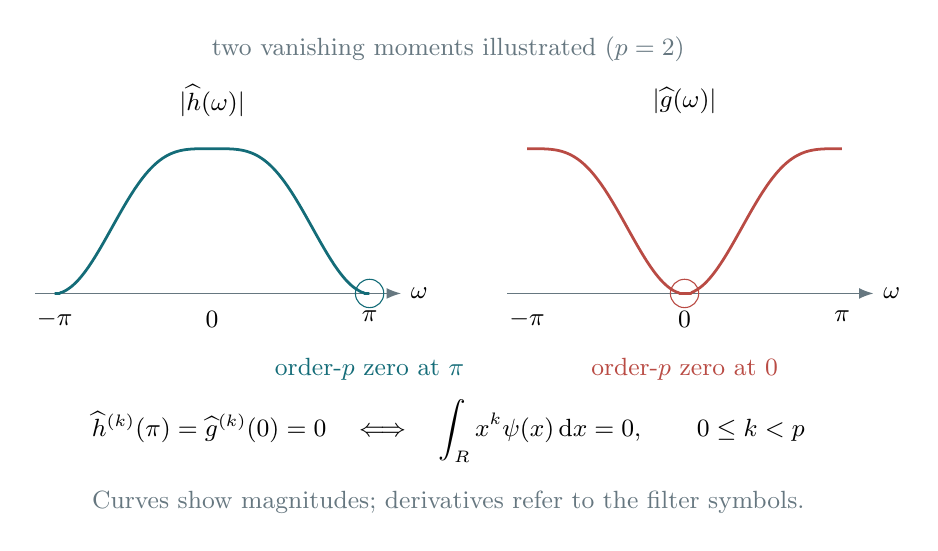
\begin{tikzpicture}[x=1cm,y=1cm]
\foreach \s/\name in {0/{|\widehat h(\omega)|},6/{|\widehat g(\omega)|}} {\begin{scope}[shift={(\s,0)}]
\draw[axis] (-2.25,0)--(2.4,0) node[right] {$\omega$};
\foreach \x/\lab in {-2/{-\pi},0/0,2/\pi} {\node[below] at (\x,-.1) {$\lab$};}
\node at (0,2.45) {$\name$};
\end{scope}}
\draw[curve,domain=-2:2,samples=201] plot (\x,{1.3*sqrt(2*(1-sin(45*\x)^2)^2*(1+2*sin(45*\x)^2))});
\draw[signalred,line width=1pt,domain=-2:2,samples=201] plot ({6+\x},{1.3*sqrt(2*sin(45*\x)^4*(3-2*sin(45*\x)^2))});
\draw[accent] (2,0) circle(.18);\draw[signalred] (6,0) circle(.18);
\node[accent,anchor=north] at (2,-.7) {order-$p$ zero at $\pi$};
\node[signalred,anchor=north] at (6,-.7) {order-$p$ zero at $0$};
\node at (3,-1.75) {$\widehat h^{(k)}(\pi)=\widehat g^{(k)}(0)=0\quad\Longleftrightarrow\quad\displaystyle\int_{\mathbb R}x^k\psi(x)\,\mathrm{d}x=0,\qquad 0\leq k<p$};
\node[muted,font=\small] at (3,-2.65) {Curves show magnitudes; derivatives refer to the filter symbols.};
\node[muted] at (3,3.1) {two vanishing moments illustrated ($p=2$)};
\end{tikzpicture}
\end{document}
